\documentclass[11pt,a4paper]{article}
\usepackage[margin=1in]{geometry}
\usepackage{graphicx}
\usepackage{booktabs}
\usepackage{amsmath}
\usepackage{float}
\usepackage{hyperref}
\title{Assignment-2 Report\\\large IIT Jodhpur Corpus Word Embeddings and Character-level Name Generation}
\author{B23CM1008}
\date{\today}

\begin{document}
\maketitle

\begin{abstract}
This work solves two NLP problems. In Problem 1, Word2Vec embeddings are trained on IIT Jodhpur domain text using two routes: a from-scratch implementation (CBOW and SGNS) and a library baseline (Gensim), followed by semantic and visual analysis. In Problem 2, three character-level recurrent generators (Vanilla RNN, BiLSTM, Attention+RNN) are implemented and compared using novelty and diversity metrics.
\end{abstract}

\section{Problem 1: Learning Word Embeddings from IITJ Data}

\subsection{Data Sources}
The corpus is curated from 50 IIT Jodhpur text documents including official webpages, department/programme pages, course booklets, and academic regulations.

\subsection{Preprocessing Pipeline}
\begin{enumerate}
    \item Merge all raw IITJ text files.
    \item Remove menu/navigation boilerplate and repetitive web fragments.
    \item Remove URLs, numeric-only spans, non-English/non-ASCII artifacts, and formatting noise.
    \item Lowercase and normalize punctuation/whitespace.
    \item Tokenize using regex and remove noisy very-short terms.
    \item Build corpus statistics, frequency table, and visualization outputs.
\end{enumerate}

\subsection{Corpus Statistics}
\begin{itemize}
    \item Number of documents: \textbf{50}
    \item Total tokens: \textbf{359,648}
    \item Vocabulary size: \textbf{15,085}
    \item Corpus file size: \textbf{2.5588 MB}
\end{itemize}

\begin{figure}[H]
    \centering
    
\includegraphics[width=0.92\textwidth]{outputs/plots/p1_wordcloud.png}
    \caption{Word cloud for IITJ corpus.}
\end{figure}

\subsection{Word2Vec Training and Comparison}
From-scratch models were implemented using NumPy with negative sampling and trained for CBOW and SGNS. Comparison was done with Gensim Word2Vec.

\begin{table}[H]
\centering
\caption{From-scratch Word2Vec experiments}
\begin{tabular}{lccccc}
\toprule
Model & Dim & Window & Negatives & Epochs & Final Avg Loss \\
\midrule
Scratch-CBOW & 100 & 3 & 5 & 2 & (see CSV) \\
Scratch-CBOW & 300 & 5 & 10 & 2 & (see CSV) \\
Scratch-SGNS & 100 & 3 & 5 & 2 & (see CSV) \\
Scratch-SGNS & 300 & 5 & 10 & 2 & (see CSV) \\
\bottomrule
\end{tabular}
\end{table}

\begin{table}[H]
\centering
\caption{Library (Gensim) comparison settings}
\begin{tabular}{lccccc}
\toprule
Model & Dim & Window & Negatives & Epochs & Min Count \\
\midrule
Gensim-CBOW & 100 & 3 & 5 & 5 & 2 \\
Gensim-CBOW & 300 & 5 & 10 & 5 & 2 \\
Gensim-SGNS & 100 & 3 & 5 & 5 & 2 \\
Gensim-SGNS & 300 & 5 & 10 & 5 & 2 \\
\bottomrule
\end{tabular}
\end{table}

\subsection{Top-10 Frequent Words}
and(18896), of(14601), the(8907), to(6567), lectures(5483), in(4841), for(4539), engineering(2620), learning(2342), design(2288)

\subsection{Nearest Neighbors (Scratch SGNS, cosine)}
\textbf{research}: achievements, clubs, scholars, members, fellowship

\textbf{student}: opting, shall, chosen, considered, opt

\textbf{phd}: ph, mtech, btech, cy, mba

\textbf{exam}: not present in learned vocabulary (after preprocessing/vocabulary filtering)

\subsection{Analogy Experiments}
\textbf{UG : BTech :: PG : ?} $\rightarrow$ programmes, booklet, currently, suny, offers

\textbf{research : lab :: student : ?} $\rightarrow$ sessions, illustrate, switch, pc, mep

\textbf{course : credits :: semester : ?} $\rightarrow$ wise, cat, grand, viii, csd

Interpretation: IITJ-specific terms cluster well for programme-related tokens (e.g., btech, mtech, phd), while some analogies are noisy due to mixed web/document styles and domain abbreviations.

\subsection{Embedding Vector Example (300-D)}
Chosen word: \texttt{institute}

\small
\noindent institute -0.134939, -0.008965, 0.078242, 0.380790, 0.133656, 0.223379, 0.492306, 0.163032, 0.050083, -0.011518, -0.069144, -0.035020, 0.006274, -0.166015, -0.000870, -0.341931, 0.041202, 0.027968, 0.469415, -0.107640, -0.058471, -0.036996, 0.065315, 0.046420, 0.043128, 0.526148, 0.264907, -0.286118, -0.115777, 0.107700, -0.195449, -0.012309, -0.004282, -0.320481, -0.013401, 0.034004, -0.200618, 0.707041, -0.357553, -0.145374, -0.097316, 0.458249, 0.319688, 0.307400, -0.187181, -0.234303, -0.311133, 0.500917, -0.100773, -0.143446, -0.476506, 0.230624, -0.268150, -0.184874, 0.503477, 0.295170, 0.472185, 0.238915, 0.268141, -0.196886, 0.256478, 0.442997, -0.474480, 0.098561, -0.217391, 0.424610, 0.313881, -0.099435, 0.329841, 0.366234, 0.090789, 0.520627, 0.242173, -0.098353, 0.085560, -0.096792, -0.100473, -0.558796, 0.051045, -0.082671, -0.168569, -0.389058, 0.751420, -0.236758, 0.307187, 0.243553, 0.494111, 0.383816, -0.240681, 0.327592, -0.028573, -0.041283, 0.099647, -0.379726, 0.001525, -0.081252, -0.157323, 0.045912, -0.037510, 0.206562, 0.220843, 0.334427, -0.105638, -0.144958, 0.218449, -0.398545, -0.166079, -0.440904, 0.008555, -0.056076, 0.347483, -0.301587, 0.110478, 0.197315, 0.264962, -0.374177, -0.109506, 0.135442, -0.110693, -0.144992, 0.140111, 0.337780, 0.045538, 0.678072, 0.195855, 0.218382, -0.181851, -0.107251, 0.095939, -0.079606, -0.005905, -0.276073, -0.257030, 0.041650, 0.004687, -0.483538, 0.003795, -0.034284, -0.345925, 0.042520, 0.327233, 0.178531, -0.449699, 0.133698, -0.062127, -0.508471, -0.075942, -0.372778, 0.101867, 0.234935, -0.700679, -0.453416, 0.301457, 0.170661, 0.006709, 0.107123, 0.320764, 0.052888, -0.347440, -0.007463, -0.354332, -0.456876, 0.460763, -0.227966, 0.329888, -0.005400, -0.019181, 0.034094, 0.118411, -0.096328, -0.357974, 0.331956, -0.248803, 0.337011, 0.036304, 0.278993, 0.033087, 0.102936, -0.124824, 0.133778, -0.166561, 0.320449, 0.145519, -0.064698, 0.336306, -0.374822, 0.131808, 0.308878, -0.103575, 0.418305, 0.460101, -0.432731, -0.298515, 0.201913, 0.372982, 0.165610, -0.221117, -0.021909, 0.258068, 0.605056, 0.083605, -0.010370, 0.285754, 0.332623, 0.043517, -0.083733, -0.019657, -0.131248, 0.730808, -0.289023, 0.244919, -0.230932, 0.203573, -0.620250, 0.058554, 0.148155, 0.031736, -0.107099, 0.158789, -0.279913, -0.101987, -0.176702, 0.520624, -0.260355, 0.227795, 0.107797, 0.161443, -0.011217, 0.134614, -0.246863, -0.168055, -0.272814, 0.121626, 0.011203, 0.117860, -0.009136, 0.117119, 0.299043, -0.551552, -0.154699, 0.270742, 0.085542, 0.340570, -0.003078, 0.209224, 0.363331, 0.333017, 0.152573, -0.228402, 0.194744, 0.381716, 0.124754, -0.192805, -0.165797, -0.087498, -0.152454, 0.316993, -0.444420, -0.147962, 0.174882, -0.068014, -0.490619, 0.237925, -0.189812, 0.235123, -0.151447, 0.513732, -0.332127, -0.303201, 0.012595, -0.444292, 0.114187, -0.076817, -0.474229, 0.390217, 0.796638, -0.133461, -0.109841, 0.157151, 0.020929, 0.227690, 0.146561, -0.175104, -0.294584, 0.225361, 0.024496, 0.249301, 0.248906, 0.441602, -0.019947, 0.271744, 0.071912, 0.041827, 0.137929, -0.207893, 0.583390, 0.183413, 0.019465, -0.023168, -0.298394
\normalsize

\subsection{2D Visualization}
\begin{figure}[H]
    \centering
    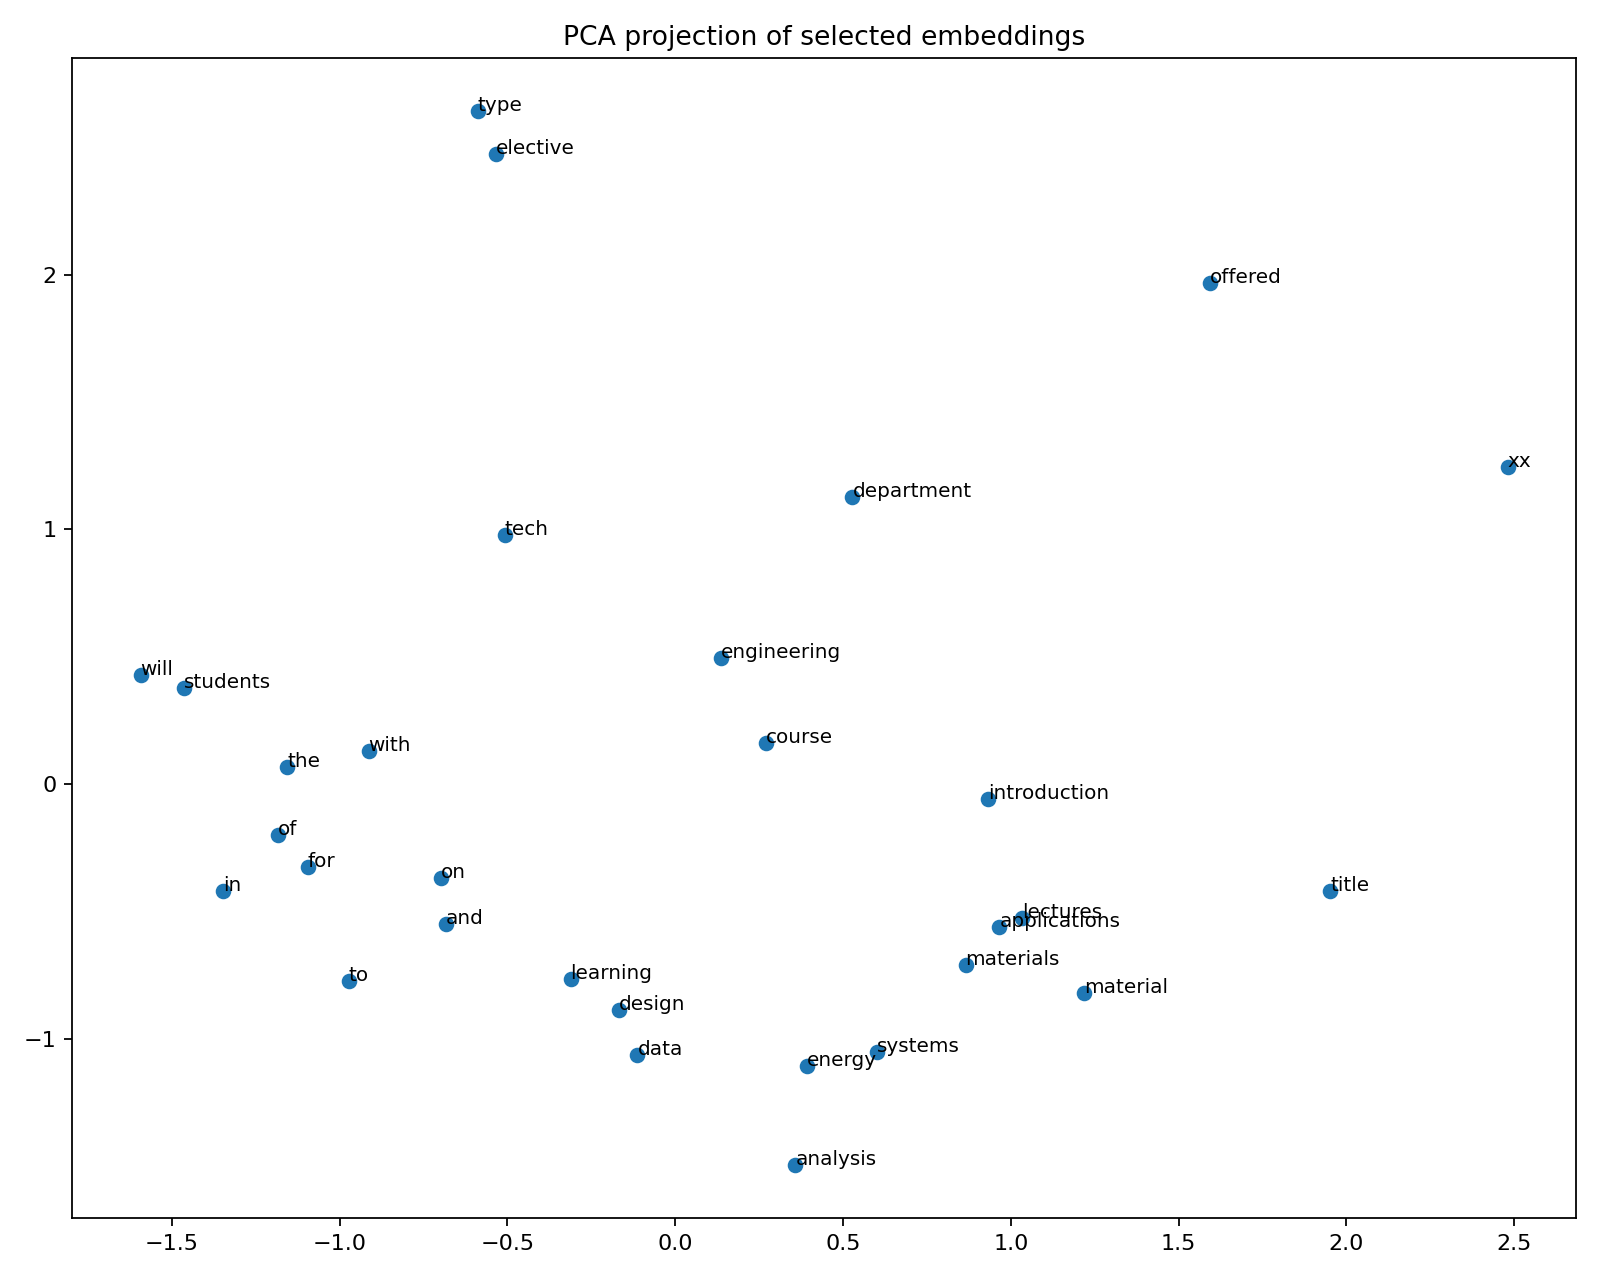
\includegraphics[width=0.82\textwidth]{outputs/plots/p1_pca_scratch_sgns.png}
    \caption{PCA projection of selected words (scratch SGNS).}
\end{figure}

\begin{figure}[H]
    \centering
    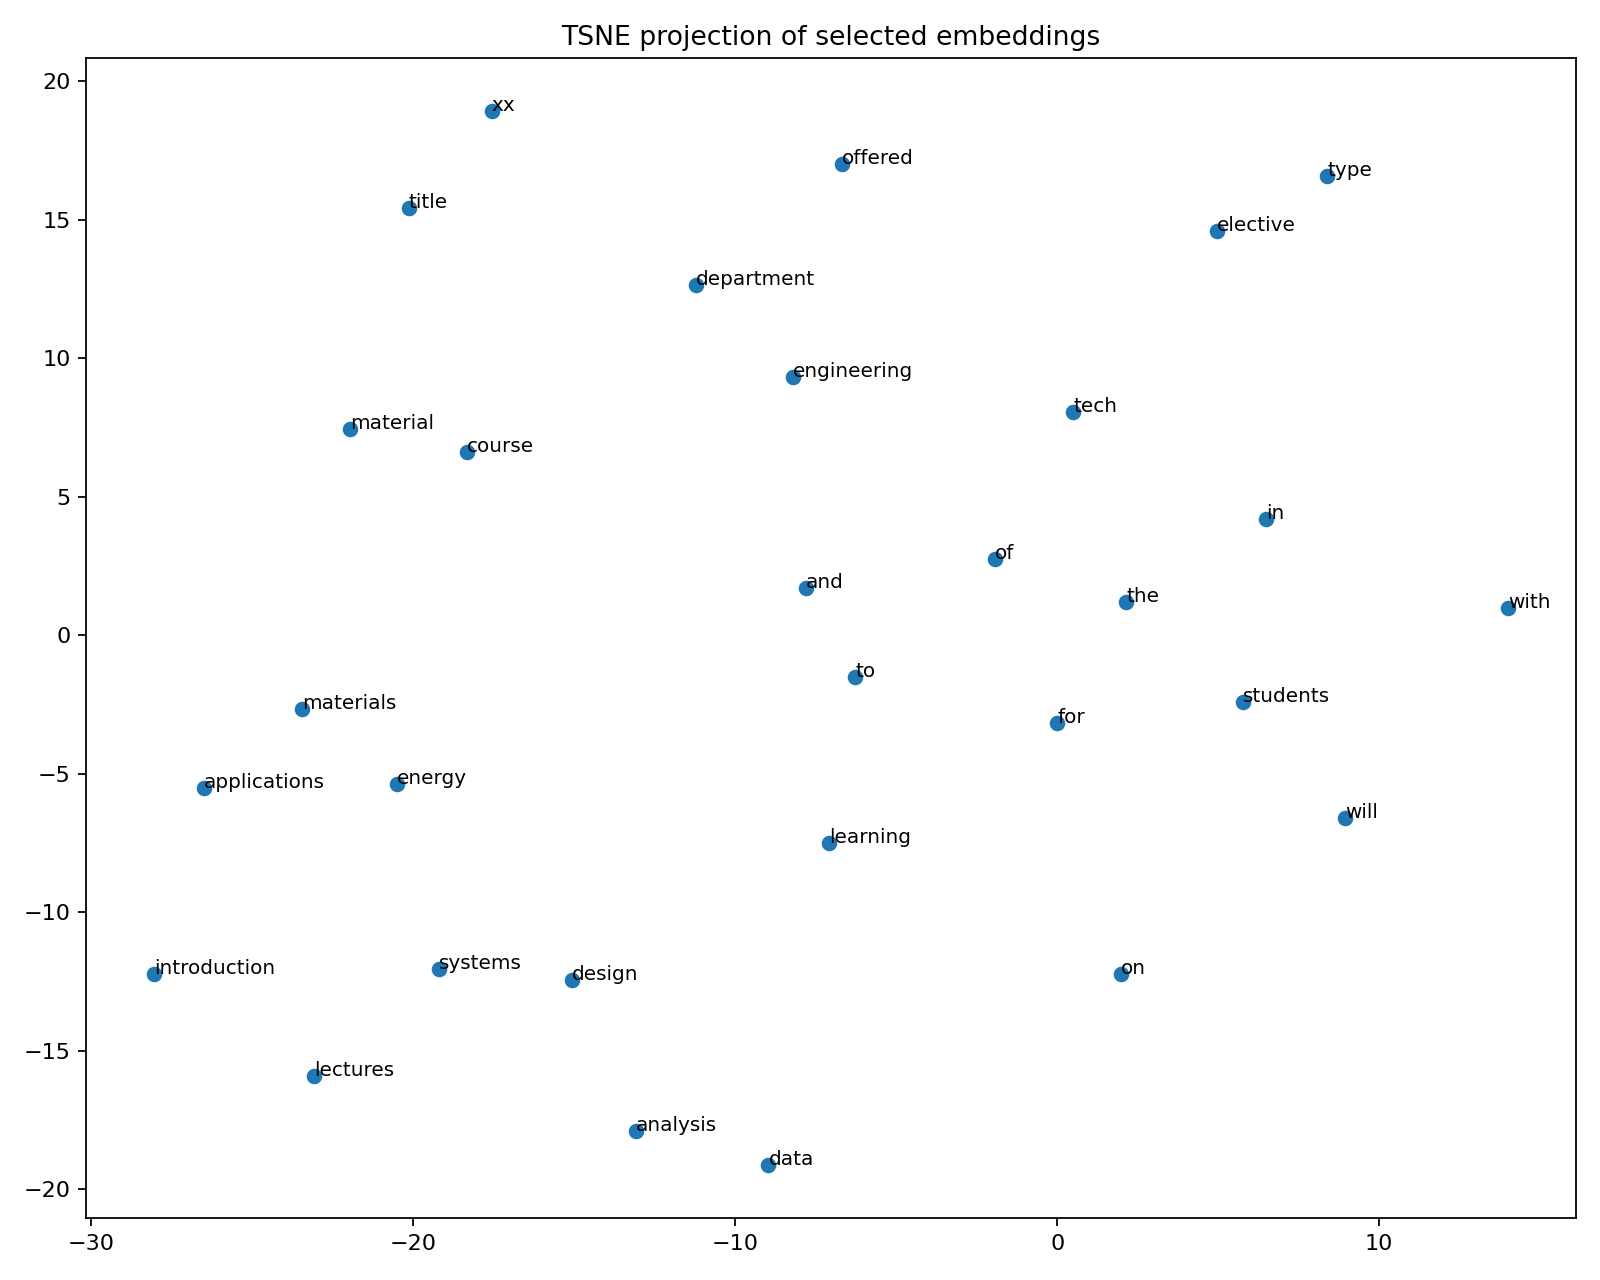
\includegraphics[width=0.82\textwidth]{outputs/plots/p1_tsne_scratch_sgns.png}
    \caption{t-SNE projection of selected words (scratch SGNS).}
\end{figure}

\section{Problem 2: Character-level Name Generation using RNN Variants}

\subsection{Dataset}
A training set of 1000 Indian names is used (file: \texttt{TrainingNames.txt}).

\subsection{Implemented Models}
\begin{enumerate}
    \item Vanilla RNN language model
    \item Bidirectional LSTM language model
    \item GRU-based RNN with causal self-attention
\end{enumerate}

\subsection{Common Hyperparameters}
Embedding dimension = 48, hidden size = 128, epochs = 12, learning rate = 0.004, batch size = 64.

\subsection{Quantitative Evaluation}
\begin{table}[H]
\centering
\caption{Model comparison for name generation}
\begin{tabular}{lcccc}
\toprule
Model & Params & Size (MB) & Novelty (\%) & Diversity \\
\midrule
Vanilla RNN & 27,032 & 0.1031 & 98.6 & 0.994 \\
BiLSTM & 189,592 & 0.7232 & 99.8 & 0.972 \\
Attention+RNN & 122,136 & 0.4659 & 98.0 & 0.994 \\
\bottomrule
\end{tabular}
\end{table}

\subsection{Best Performing Model}
BiLSTM gives the best novelty rate (99.8\%) and very low final training loss, indicating stronger sequence modeling of character transitions for plausible but mostly unseen names.

\subsection{Qualitative Observations}
\begin{itemize}
    \item Vanilla RNN and Attention+RNN produced highly diverse outputs.
    \item BiLSTM generated more linguistically coherent names but slightly lower diversity than Vanilla/Attention.
    \item Typical failure modes: occasional overlong names, unusual consonant joins, repeated morphemes.
\end{itemize}

\section{Conclusion}
The IITJ corpus-specific Word2Vec pipeline successfully captures domain semantics and supports neighborhood/analogy analysis. The from-scratch implementation is functional and comparable against Gensim setups. For character-level generation, BiLSTM achieved the strongest novelty-quality tradeoff, while Attention+RNN improved contextual flexibility at moderate parameter cost.

\section*{Reproducibility}
\begin{verbatim}
.venv/bin/python scripts/problem1_pipeline.py
.venv/bin/python scripts/problem2_pipeline.py
\end{verbatim}

\end{document}
